	\documentclass[10pt,oneside]{CBFT_book}
	% Algunos paquetes
	\usepackage{amssymb}
	\usepackage{amsmath}
	\usepackage{graphicx}
% 	\usepackage{libertine}
% 	\usepackage[bold-style=TeX]{unicode-math}
	\usepackage{lipsum}

	\usepackage{natbib}
	\setcitestyle{square}

	\usepackage{polyglossia}
	\setdefaultlanguage{spanish}
	



	\usepackage{CBFT.estilo} % Cargo la hoja de estilo

	% Tipografías
	% \setromanfont[Mapping=tex-text]{Linux Libertine O}
	% \setsansfont[Mapping=tex-text]{DejaVu Sans}
	% \setmonofont[Mapping=tex-text]{DejaVu Sans Mono}

	%===================================================================
	%	DOCUMENTO PROPIAMENTE DICHO
	%===================================================================

\begin{document}

% =================================================================================================
\chapter{Gases imperfectos}
% =================================================================================================


% =================================================================================================
\section{Cuánticos --reubicar}
% =================================================================================================

Ensamble de $ \mathcal{N} $ sistemas $(k=1,2,...,\mathcal{N})$. Cada uno tiene su estado descripto por 
\[
	\Psi^k(\vb{x},t), \qquad \qquad \hat{H} \Psi^k = i\hbar \dpar{\Psi^k}{t} \quad \forall k
\]

Si son estados puros entonces 
\notamargen{Todos son la {\it misma} combinación lineal de la base.}
\[
	\Psi^k = \sum_n a_n(t) \phi_n(\vb{x}) \qquad \{ \phi_n \} \text{ set ortonormal }
\]
Un estado puro es superposición coherente de una base 
\[
	i \hbar \dpar{}{t} a_m^k = \sum_n H_{mn}a_n^k
\]

El sistema k-ésimo puede describirse a partir de $ \Psi^k $ o bien a partir de los coeficientes $ \{ a_n \}$.

Definimos un operador de densidad,
\notamargen{Promedio en el ensamble de la interferencia cuántica entre $\phi_m$ y $\phi_n$. $p_k$ es la probabilidad
del estado $k$.}
\[
	\rho_{mn} \equiv \sum_{k=1}^{\mathcal{N}} p_k a_m^k (a_n^k)^*
\]
el cual proviene de 
\[
	\hat{\rho}_{mn} = \sum_{k=1}^{\mathcal{N}} p_k \Ket{\Psi^k}\Bra{\Psi^k}
\]
\notamargen{¿Y los índices $mn$ capo?}

Puede verse que se cumple
\[
	i \hbar \dot{\rho} = [ \hat{H}, \hat{\rho} ],  
\]
un teorema de Liouville cuántico.
 
Sea el valor medio de $ \hat{G} $
\[
	\braket{G}_{ENS} = \sum_{k=1}^{\mathcal{N}} p_k \braket{G}_k = 
	\sum_{k=1}^{\mathcal{N}} p_k \braket{\Psi^k|\hat{G}|\Psi^k}_k = 
	\sum_k p_k \int \sum_i a_i^{k*}\phi_i^* \hat{G}\sum_j a_j^k\phi_j dx
\]
\[
	\braket{G}_{ENS} = \sum_k p_k \sum_i \sum_j a_i^{k*}  a_j^k \int \phi_i^* G \phi_j dx =
	\sum_i \sum_j \left( \sum_k p_k a_i^{k*}  a_j^k \right) G_{ij}
\]
\[
	\braket{G}_{ENS} = \sum_i \sum_j \rho_{ij} G_{ij} = 
	\text{ Traza }(\hat{\rho}\hat{G}) = \sum_i [\rho G]_{ii}
\]

Ahora, si el conjunto $\{ \phi_n \}$ fuesen autoestados de $\hat{G}$ entonces 
\[
	\int dx \phi_i^* G \phi_j = \int dx \phi_i^* \phi_j g_j = \delta_{ij} g_j = g_i
\]
\[
	\braket{G}_{ENS} = \sum_k p_k \sum_i a_i^{k*}  a_i^k g_i = 
	\sum_k p_k \sum_i |a_i^k|^2 g_i
\]

La matriz densidad $\hat{\rho}$ se define de modo que sus elementos $\rho_{ij}$ resultan 
\[
	\braket{\phi_i|\hat{\rho}|\phi_j} = \sum_{k=1}^{\mathcal{N}} p_k \braket{\phi_i|\Psi^k} \braket{\Psi^k|\phi_j} =
	\sum_{k=1}^{\mathcal{N}} p_k \int dx \phi^*_i \sum_l a_l^k \phi_l \int dx' \phi_j \sum_m a_m^{k*} \phi_m^*
\]
\[
	\braket{\phi_i|\hat{\rho}|\phi_j} = 
	\sum_{k=1}^{\mathcal{N}} p_k \sum_l \sum_m a_l^k a_m^{k*} \int dx \phi^*_i \phi_l \int dx' \phi_j \phi_m^* =
	\sum_{k=1}^{\mathcal{N}} p_k \sum_l \sum_m a_l^k a_m^{k*} \delta_{il}\delta_{jm}
\]
\[
	\rho_{ij} = \sum_k p_k a_i^k a_j^{k*}
\]

El primer postulado de la QSM es asegurarse de que $\rho_{ij} \propto \delta_{ij} $, es decir que
EN PROMEDIO no hay correlación entre funciones $\{ \phi_i \}$ para diferentes miembros $k$ del ensamble.
El elemento $\rho_{ij}$ es el promedio en el ensamble de la interferencia entre $\phi_i$ y $\phi_j$.


En la práctica los ensambles serán mezcla, una superposición de estados puros pero incoherente, de modo
que 
\notamargen{Es muy difícil preparar un ensamble puro.}
\[
	\hat{\rho} = \sum_{k=1}^{\mathcal{N}} p_k \Ket{\Psi^k}\Bra{\Psi^k} \qquad p_k \geq 0 \quad \sum_k p_k = 1 
\]
donde $p_k$ serán las {\it abundancias relativas} de los estados puros $\Psi^k$.

Para un ensamble puro sería
\[
	\hat{\rho} = \Ket{\Psi}\Bra{\Psi}
\]
donde no hay supraíndice $k$ puesto que todos son el mismo estado.

Un estado puro puede escribirse 
\[
	\Psi^k = \sum_n a_n \phi_n, \quad \text{ o bien }\quad \Ket{\Psi^k} = \sum_n a_n \Ket{\phi_n}
\]
y sabemos que el valor de expectación será
\[
	\braket{A}_k = \braket{\Psi^k|\hat{A}|\Psi^k} = \int dx \Psi^{k*} A \Psi^k
\]

Un estado mezcla será en cambio 
\be
	\Ket{\xi} \cong \sum_n p_n\Ket{\phi_n}
	\label{estado_mezcla}	
\ee
donde $\sum_n p_n =1$ y $p_n \in \mathbb{R}>0$. Pero $\Ket{\xi} $ no es un estado de sistema como $\Psi^k$ pués
\be
	\Ket{\xi} \neq \sum_n c_n\Ket{\phi_n}
	\label{falso_mezcla}
\ee
no hay cambio de base que lleve \eqref{estado_mezcla} al miembro derecho de \eqref{falso_mezcla}.
Entonces
\[
	\braket{A}_\xi \neq \braket{\xi|\hat{A}|\xi}
\]

Pero como en la práctica lo que se tiene son estados mezcla, la matriz de densidad $\hat{\rho}$ permite trabajar
con ellos tranquilamente.

Sea que evaluamos el valor medio de $ \hat{G} = \hat{\Ham} $ que será la energía $\braket{E}$ en autoestados de 
$ \hat{\Ham} $.
\[
	\braket{\hat{\Ham}}_{ENS} = \braket{E} = \sum_k p_k \sum_i \sum_j a_i^{k*} a_j^k \int \phi_i^* \phi_j E_j =
	\sum_k p_k \sum_j a_j^{k*} a_j^k E_j
\]
\[
	\braket{E} = \sum_k p_k \sum_j a_j^{k*} a_j^k E_j = \sum_j \left( \sum_k p_k a_j^{k*} a_j^k \right) E_j =
	\sum_j \rho_{jj} E_j
\]

Se tiene que $ \hat{\rho} $ es diagonal para un operador $\hat{G}$ tal que utilizamos la base de autoestados.

Querremos que esto valga para cualquier base entonces necesitaremos que las fases sean números aleatorios:
\[
	\rho_{ij} = \sum_k^{\mathcal{N}} p_k a_i^{k*} a_j^k = 
	\sum_k^{\mathcal{N}} p_k | a_i^k | | a_j^k |\euler^{i( \theta_i^k - \theta_j^k )}
\]
y asi además son equiprobables (microcanónico) los estados base accesibles,
\[
	p_k = \frac{1}{\mathcal{N}} \qquad \text{ y } \qquad |a^k_i| = |a_i| \quad \forall k
\]
y asimismo pedimos que para cada miembro del ensamble la amplitud sea la misma, se tiene 
\[
	\rho_{ij} = | a_i | | a_j | \frac{1}{\mathcal{N}} \sum_k^{\mathcal{N}} \euler^{i( \theta_i^k - \theta_j^k )}
	= | a_i | | a_j | \delta_{ij}
\]
donde se han usado fases al azar, de modo que 
\[
	\rho_{ij} = | a_i |^2 \delta_{ij} = \rho_i \delta_{ij}
\]
\notamargen{Esto no está consistente: colapsas la delta o no, papi?}
y entonces 
\[
	\begin{cases}
	 \rho_i = \displaystyle{ \frac{1}{\Gamma} }\\
	 \rho_i = 0
	\end{cases}
\]

Entonces $ \rho_i $ será la probabilidad del estado de base $ \phi_i $. Se sigue que el operador densidad del
microcanónico puede escribirse 
\[
	\hat{\rho} = \sum_i | a_i |^2 \Ket{\phi_i}\Bra{\phi_i}
\]
de manera que es una superposición incoherente de estados de la base $\{ \phi_i \}$
\[
	\hat{\rho} = \sum_i \rho_i \Ket{\phi_i}\Bra{\phi_i}
\]
y al final del día
\[
	\rho_{kl} = \braket{ \phi_k | \hat{\rho} | \phi_l } = \sum_i \rho_i 
	\braket{ \phi_k | \phi_i }  \braket{ \phi_i | \phi_l } = \sum_i \rho_i \delta_{ki} \delta_{il} = 
	\rho_k \delta_{kl}
\]

\[
	\Omega = 1 \text{ ensamble puro } \qquad \qquad S = k\log \Omega = 0
\]
\[
	\rho_{mn} = \frac{1}{\mathcal{N}} \sum_k^{\mathcal{N}} a_m^{k*} a_m^k = a_m a_n^* 
\]
si es la misma $\Psi \forall k$ el sistema se halla en una combinación lineal de $\phi_n$, o bien
\[
	\rho_{mn} = |a_m|^2 \delta_{mn}
\]
el sistema se halla en un único autoestado $ \phi_n $

\[
	\Omega > 1 \text{ ensamble mezcla }
\]

\subsection{Resumen formalismo}

\[
	\rho_{ij} = \rho_i \delta_{ij}
\]
\[
	\rho_i = \frac{1}{\Omega} \qquad \text{ Microcanónico }
\]
\[
	\rho_i = \frac{\euler^{-\beta E_i}}{Q_N(V,T)}  \qquad  \text{ Canónico }
\]
\[
	\rho_i = \frac{\euler^{-\beta E_i + \beta \mu N_i }}{\Xi(z,V,T)}  \qquad  \text{ Gran canónico }
\]

\[
	\hat{\rho} = \sum_i \Ket{ \phi_i } \rho_i \Bra{ \phi_i } \qquad \qquad \text{ Traza }(\hat{\rho} ) =
	1 \text{ bien normalizado }
\]
\[
	\hat{\rho} = \frac{1}{\Omega} \sum_i^{\text{ACC}} \Ket{ \phi_i } \Bra{ \phi_i } = 
	\frac{1}{\Omega} \hat{\mathbb{1}}^{\text{ACC}}  \qquad \text{ Tr }(\hat{\rho} ) = 1 
\]
donde $ \hat{\mathbb{1}}^{\text{ACC}}  $ es una indentidad con 0 para los sitios de la diagonal donde no hay
estado accesible. Luego $ \text{ Traza }(\hat{\mathbb{1}}^{\text{ACC}})  = \Omega $. Para los otros dos casos,
\[
	\hat{\rho} = \frac{\euler^{-\beta E_i}}{Q_N(V,T)}  \sum_i^{\text{ACC}} \Ket{ \phi_i } \Bra{ \phi_i } = 
	\frac{\euler^{-\beta E_i}}{Q_N(V,T)} \hat{\mathbb{1}}^{\text{ACC}} 
	\qquad \text{ Tr }(\hat{\rho} ) = \frac{1}{Q_N} \text{ Tr }( \euler^{-\beta E_i} \hat{\mathbb{1}}^{\text{ACC}} )
\]
\[
	\hat{\rho} = \frac{\euler^{-\beta E_i + \beta \mu N_i }}{\Xi(z,V,T)} 
	\sum_i^{\text{ACC}} \Ket{ \phi_i } \Bra{ \phi_i } = 
	\frac{\euler^{-\beta E_i + \beta \mu N_i }}{\Xi(z,V,T)} \hat{\mathbb{1}}^{\text{ACC}} 
	\qquad \text{ Tr }(\hat{\rho} ) = 
	\frac{1}{\Xi} \text{ Tr }( \euler^{-\beta E_i + \beta \mu N_i } \hat{\mathbb{1}}^{\text{ACC}} ) 
\]

El conteo de estados se hace cuánticamente de modo que no hay paradoja de Gibbs. Los estados accesibles en el
microcanónico $ (\Omega) $ son tales que sus probabilidad es 
\[
	| a_i |^2 = \frac{1}{\Omega} \quad \forall i \text{ accesible }
\]
Serán aquellos de la base $ \{ \phi_i \} $ en cuestión tales que la energía resulte vale entre $E$ y $E+\Delta E$.

Los dos postulados
\begin{itemize}
 \item i) Equiprobabilidad
 \item ii) Fases al azar
\end{itemize}
aseguran que no hay correlación entre las funciones $ \{ \phi_i \} $ (en promedio).


% =================================================================================================
\section{Gases reales}
% =================================================================================================

Función canónica de un gas real. Surge una integral configuracional
\[
	Z_N =  \int d^3q_1 ... d^3q_N \euler^{ - \beta \sum_{i<j} V_{ij} }
\]
En el gran canónico tenemos $ \Xi( Z_N ) $. Potencial de Lenard-Jones
\[
	\frac{1}{r^{12}} - \frac{1}{r^{6}}
\]

Definimos $ f_{ij} = \euler^{-\beta V_{ij}} - 1 $ y expresamos todo en términos de $ f_{ij} $.
Esta última tiene el mismo rango que el potencial de interacción.
De alguna manera esto que haremos es un desarrollo en serie del potencial de interacción.

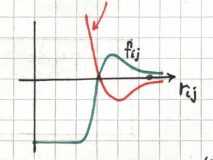
\includegraphics[scale=0.5]{images/1606329591.jpg}

Estudiamos con los N-grafos.

Consideramos un hamiltonianao
\[
	H = \sum_i^N \frac{ p^2 }{2m} + \sum V_{ij},
\]
donde $V_{ij}$ depende de $|r_i-r_j|$. Es un modelo clásico pero consideramos interacción.
La función de partición no se factoriza como el producto de funciones de una partícula justamente
debido a la interacción.

Metemos grafos ahora y llegaremos a una expresión para los coeficientes del virial.
El gas real lo estudiamos clásicamente, entonces 
\[
	Q_N = \frac{1}{N! h^{3N} } \int  d^{3N}q d^{3N}p  \euler^{ - \beta H(p,q) }
\]
si bien aparece $h$ (constante de Planck) no hablamos de funciones de onda; como sí sucede en una
expansión cuántica.
Se integra en los momentos y resulta
\[
	Q_N = \frac{1}{N! \lambda^{3N} } \int  d^{3N}q  \euler^{ - \beta \sum_{i<j} v_{ij} }
\]
donde $\lambda$ absorbe muchas constantes. Luego,
\[
	Q_N(V,T) = \frac{ Z_N }{ N! \lambda^{3N}},
\]
con $ Z_N $ la función de partición o integral configuracional.

El kid de la cuestión será hallar expresión para $Z_N$ que sea manejable. Pasaremos al gran canónico
\[
	\Xi(z,V,T) = \sum_{N=0}^\infty \: \Frac{z}{\lambda^3}^N \frac{ Z_N }{ N! }
\]
y usaremos la definición $f_{ij}$ que es de Mayer (1937) y vemos que sucede que 
\begin{itemize}
 \item $f_{ij}=0$ si $v_{ij}=0$
 \item No diverge
 \item $f_{ij} \sim 0$ con $r \gg r_0 $
 \item $f_{ij} \approx 0$ con $ k T \gg v_{ij}$ (altas temperaturas)
\end{itemize}

Todo esto parece razonable para los límites conocidos

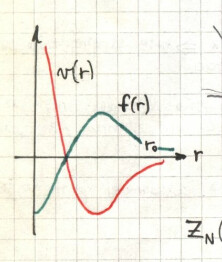
\includegraphics[scale=0.4]{images/1606337067.jpg}

La integral configuracional es un producto entre números de pares de partículas posibles
\[
	Z_N = \int  d^{3N}q \prod_{i<j} ( 1 + f_{ij} ),
\]
la cual tendrá $ (N-1)N/2 $ productos y $ 2^{N(N-1)/2} $ términos sumando de modo que serán esa cantidad
de integrales
\notamargen{Cada grafo puede verse en una matriz de adyacencias $M_{ij}$}
\begin{center}
\begin{tabular}{cc}
N=2 $ \to $ & $1$ producto y $2^1$ términos \\
N=3 $ \to $ & $3$ productos y $2^3=8$ términos \\
N=4 $ \to $ & $6$ productos y $2^6=64$ términos \\
N=10 $ \to $ & $45$ productos y $2^{45} \cong 3.5\cdot 10^{13}$ términos 
\end{tabular}
\end{center}
O sea que la intgral es una cosa del tipo 
\[
	Z_N = \int d^{3N}r \left[ 1 + (f_{12} + f_{13} + f_{23} + ... )
	+ ( f_{12} f_{13} + f_{12} f_{11} + ... ) + ... \right]
\]
y para hacer esta cuenta se asocia una integral con un grafo de $N$ partículas.

Por ejemplo tenemos un grafo de cuatro partículas y un grafo que se factoriza porque hay partes
disconexas

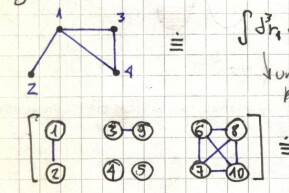
\includegraphics[scale=0.4]{images/1606337071.jpg}

que representan un 4-grafo
\[
	\int d^3r_1  d^3r_2 d^3r_3 d^3r_4 f_{12} f_{13} f_{34} f_{14},
\]
y un 10-grafo
\[
	\int d^3r_1 ... d^3r_{10} f_{39} f_{67} f_{68} f_{12} ...
\]

La factorización de este lleva a 

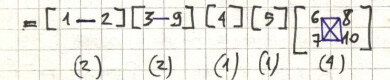
\includegraphics[scale=0.4]{images/1606337077.jpg}

donde cada uno es un {\it cluster} (racimo). Un $\ell-$cluster es un grupo de $\ell$ partículas que están
conectadas de modo que no se puede descomponer.

Cada grafo puede descomponerse en clusters y la función de partición puede epxresarse como la suma
de todos los posibles distintos grafos donde cada grafo puede factorizarse en clusters.

Es conveniente definir entonces una integral de cluster (racimo) que son las $b_\ell$



Cada uno de los N-grafos (integrales) puede factorizarse en l-racimos (l-grafo conexo).
\notamargen{Cada integral puede verse como un grafo. Anoté que esto puede verse bien
del libro de Pathria.}

La forma de asignar los índice será:
\[
	\frac{ N! }{[ (1!)^{m_1} \: (2!)^{m_1} \: ... ] m_1! \: m_2! \: ...}
\]
donde el corchete son permutaciones en el racimo y lo otro son permutaciones entre racimos.
Al final del día será,
\[
	\frac{PV}{kT} = \frac{ \sum \: z^\ell b_\ell }{ \sum \: \ell z^\ell b_\ell  }.
\]

Un dado N-grafo, por ejemplo

DIBUJO=
\begin{multline*}
	\int d^3r_1 d^3r_2 f_{12} \int d^3r_3  \int d^3r_4 d^3r_6 f_{46} \int d^3r_5 \times  \\
	\int d^3r_7 d^3r_8 d^3r_9 d^3r_{10} f_{78} f_{79} f_{710} f_{89} f_{910} 
\end{multline*}
tiene dos 1-racimo, dos 2-racimos y un 4-racimo.

\notamargen{Términos $f_{ij}$ son los links en el lenguaje de grafos.}
Un dado l-racimo tendrá al menos l-1 términos $f_{ij}$ para asegurar la conexión. El máximo será $l(l-1)/2$.
Se cumple 
\be
	N = \sum_{l=1}^N  \; l \cdot m_l \quad \text{ suma en racimos }
	\label{constraint}
\ee
siendo $l$ el número de partículas del racimo y $m_l$ el número de l-racimos y sujeta a
\[
	N = 1 \cdot 2 + 2 \cdot 2 + 4 \cdot 1 = 10 \qquad  \{ m_l \} = ( 2,2,0,1,0,0,0,0,0,0 )
\]

DIBUJO 

Claramente separando en racimos cuento las partículas con \eqref{constraint}.

\notamargen{Cada N-grafo se divide en varios l-racimos. Un l-racimo tendrá de 1 a N partículas.}
DIBUJO 

Pero el set $ \{ m_l \} $ tiene degeneración pues es equivalente a este otro arreglo de racimos.

Se definen las integrales de racimo como 
\[
	b_l = \frac{1}{l! \lambda^{3l-3} V} \left[ \text{ suma de todos los l-racimos posibles }\right]
\]
donde sumar los l-racimos es en todas las configuraciones de l-bolas conexas DIBUJITO.
\[
	b_1 = \frac{1}{1! \lambda^0 V} \int d^3r_1 \leftarrow \sum \boxed{1} 
\]
\notamargen{Cambiar los boxed por circled!!!}
\[
	b_2 = \frac{1}{2! \lambda^3 V} \int d^3r_1 d^3r_2  f_{12} \leftarrow \sum \boxed{1} -- \boxed{2}
\]
\begin{multline*}
	b_3 = \frac{1}{3! \lambda^6 V} \int d^3r_1 d^3r_2 d^3r_3 (f_{12}f_{23} + f_{12}f_{13} + f_{13}f_{23}+
	f_{12}f_{13}f_{23} ) \\
	\leftarrow \sum_{\text{ perm. etiqu. }} \left[ \; \boxed{\phantom{a}}-\boxed{\phantom{a}} + 
	\boxed{\phantom{a}}-\boxed{\phantom{a}}-\boxed{\phantom{a}} \; \right]
\end{multline*}

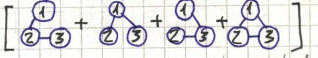
\includegraphics[scale=0.4]{images/1606337083.jpg}

Un par de cosas. Podemos definir un $b_\ell$ especial tal que 
\[
	\text{\sout{b}}_\ell(T) \equiv \lim_{V\to\infty} b_\ell(V,T) = \text{ finito }
\]
Además el $b_2$ se puede referir a coordenadas del centro de masa y así resulta
\[
	b_2 = \frac{1}{2! \lambda^3 V} \int d^3r_{12} f_{12}.
\]

Sea $ S( \{ m_l \} ) $ la suma de todos los l-racimos compatibles con el conjunto $ \{ m_l \}$
\[
	S( \{ m_l \} ) = \sum_{\text{ perm. conectores. }} \left[ \boxed{ \phantom{a} } \right]^2 \cdot 
	\left[ \boxed{ \phantom{a} }-- \right]^2 \left[ \boxed{ \phantom{a} } ---- \right]^1
\]
donde los conectores se permutan dentro de cada racimo.
\[
	Z_N = \int d^3q_1 d^3q_2 ... d^3q_N \: ( 1 + f_{12} + f_{13} + ... + f_{12}f_{13} + ... )
\]

Tenemos $ 2^{N(N-1)/2} $ integrales
\[
	Z_N = \int d^3q_1 1 + \int d^3q_2 f_{12} + ... + \int d^3q_N f_{12}f_{13} 
\]
Cada integral es un N-grafo (N bolas unidas por un número $m$ de links ($m$ es igual al número de $f_{ij}$)).

Cada N-grafo se factoriza en l-racimos y se puede escribir 
\[
	N = \sum_{l=1}^N  \; l \cdot m_l \quad \text{ suma en racimos }
\]
siendo $l$ el número de partículas en el racimo $l$ y $m_l$ el número de l-racimos. 
El conjunto $ \{ m_l \} $ es la distribución de l-racimos de un grafo
\[
	1. \text{ es } \{ m_l \} = ( N, 0, 0 , ..., 0 ) \qquad \text{ tiene $N$ 1-racimos }
\]
\[
	2.  \{ m_l \} = ( N-2, 1, 0 , ..., 0 ) \qquad \text{ tiene $N-2$ 1-racimos y $1$ 2-racimo }
\]
\[
	3. \{ m_l \} = ( N-3, 0, 1 , ..., 0 ) \qquad \text{ tiene $N-3$ 1-racimos y $1$ 3-racimo }
\]
\notamargen{ \[ N = N\cdot 1 \] \[ N = (N-2)\cdot 1 + 1 \cdot 2 \] \[ N = 1\cdot(N-3) + 3\cdot 1\]}

Sea $ S( \{ m_l \} ) $ la suma de todos los l-racimos compatibles con un conjunto $ \{ m_l \}$ dado,
\[
	S( \{ m_l \} ) = \sum_{\text{ perm. conectores. }} \left[ \boxed{ \phantom{a} } \right]^{m_1} \cdot 
	\left[ \boxed{ \phantom{a} }-- \right]^{m_2} \left[ \boxed{ \phantom{a} } ---- \right]^{m_3} \times ...
\]



Por ejemplo, para $m_3=2$ (dos 3-racimos)
\[
	\equiv 
\]
\[
	\equiv 
\]
\notamargen{Faltan los diagramáticos de estas cosas.}
y entonces 
\[
	\oplus
\]
lo que da un total de 16 términos.

Esto da el número de formas de construir un 6-grafo compuesto de dos 3-racimos

DIBUJO

Cada set $ \{ m_l \} $ define un conjunto de $ R = \sum m_l $ racimos correspondiente a un conjunto de 
N-grafos. Así:
\[
	\{ m_l \} = ( N-2, 1, 0, ..., 0 )
\]
representa

DIBUJO 

una gran cantidad de N-grafos dada por permutar etiquetas. Pero si quiero economizar cuentas similares consideraré
un factor 
\[
	\frac{1}{ 1!^{m_1} 2!^{m_2} 3!^{m_3} ... N!^{m_N} }
\]
por permutaciones de índices en cada racimo 
\[
	\frac{1}{ m_1! m_2! ... m_N! }
\]
por permutaciones de índices entre racimos iguales.

Para el ejemplo es 
\[
	\frac{1}{1!^{N-1} 2!^1} \frac{1}{(N-2)! 1!}
\]
Entonces
\[
	S( \{ m_l \} ) = \frac{1}{ 1!^{m_1} 2!^{m_2} 3!^{m_3} ... N!^{m_N} } \frac{1}{ m_1! m_2! ... m_N! }
	\left[ \boxed{ \phantom{a} } \right]^{m_1} \times \left[ \boxed{ \phantom{a} }-- \right]^{m_2} \times ...
\]
\[
	S( ( N-2, 1, 0, ..., 0 ) ) = \frac{ N(N-1) }{2!}
	\left[ \boxed{ \phantom{a} } \right]^{m_1} \times \left[ \boxed{ \phantom{a} }-- \right]^{m_2} \times
	\left[ \boxed{ \phantom{a} } ---- \right]^{m_3} \times ...
\]

Recordando 
\[
	b_l = \frac{ 1 }{ l! \lambda^{3(l-1)} V }\cdot ( \text{ Suma de todos los l-racimos } )
\]
será 
\[
	S( \{ m_l \} ) = \frac{N!}{ 1!^{m_1} 2!^{m_2} 3!^{m_3} ... N!^{m_N} } \: \prod_{l}^N \: 
	\frac{ ( l! \lambda^{3(l-1)} V \: b_l )^{ m_l } }{ m_1! m_2! ... m_N! }
\]
\[
	S( \{ m_l \} ) = N! \: \prod_{l}^N \: 
	\frac{ ( \lambda^{3(l-1)} V \: b_l )^{ m_l } }{ m_1! m_2! ... m_N! }
\]

Luego
\[
	Z_N = \sum_{\{ m_l \} } ' S( \{ m_l \} ) = N! \lambda^{3N}  \sum_{\{ m_l \} }' \prod_{l}^N 
	\frac{1}{m_l!} \Frac{ V \: b_l }{ \lambda^3 }^{m_l}
\]
\[
	Q_N = \frac{1}{N! \lambda^{3N}} Z_N = 
	\sum_{\{ m_l \} }' \prod_{l}^N \frac{1}{m_l!} \Frac{ V \: b_l }{ \lambda^3 }^{m_l}
\]
\[
	\Xi = \sum_{N=0}^\infty z^N Q_N =  \sum_{m_1=0}^\infty \sum_{m_2=0}^\infty ...  \sum_{m_N=0}^\infty
	z^N \prod_{l}^N \frac{1}{m_l!} \Frac{ V \: b_l }{ \lambda^3 }^{m_l}
\]
\[
	\Xi = \sum_{m_1=0}^\infty \sum_{m_2=0}^\infty ...  \sum_{m_N=0}^\infty
	\prod_{l}^N \frac{1}{m_l!} \Frac{ z^l V \: b_l }{ \lambda^3 }^{m_l}
\]
\[
	\Xi = \prod_{l=1}^N \sum_{m_l=0}^\infty \frac{1}{m_l!} \Frac{ z^l V \: b_l }{ \lambda^3 }^{m_l}
	= \prod_{l=1}^N \euler^{ \frac{ z^l V \: b_l }{ \lambda^3 } }
\]
\[
	\log \Xi = \sum_{l=1}^N \log\left( \euler^{ \frac{ z^l V \: b_l }{ \lambda^3 } } \right) =
	\sum_{l=1}^N  \frac{ z^l V \: b_l }{ \lambda^3 }
\]
de modo que 
\[
	\beta p = \frac{ 1 }{ \lambda^3 } \sum_{l=1}^N  z^l b_l .
\]
	
\[
	b_1 = \frac{1}{1!\lambda^{3(1-1)}V} \int d^3r = \frac{V}{\lambda^0 V} = 1
\]
\[
	b_2 = \frac{1}{2\lambda^3 V} \int d^3r d^3r' f_{rr'} = \frac{1}{2\lambda^3 V} \int d^3r \int d^3u f_u
\]
\notamargen{$r-r'= u$ y entonces $-dr'= du$.}

Tenemos, una vez más,
\[
	\Xi(z,V,T) = \euler^{ \sum_{\ell=1}^\infty \: b_\ell z^\ell V / \lambda^3 }
\]
y considerando el límite termodinámico tenemos
\[
	\frac{P}{kT} = \frac{1}{\lambda^3} \sum_{\ell=1}^\infty \: \text{\sout{b}}_\ell z^\ell
	\qquad \qquad 
	\frac{1}{v} = \frac{N}{V} = \frac{1}{\lambda^3} \sum_{\ell=1}^\infty \: \ell \: \text{\sout{b}}_\ell z^\ell
\]

desde las cuales obtenemos (también en función de la densidad)
\[
	\frac{Pv}{kT} = \sum_{\ell=1}^\infty \: a_\ell(T) \Frac{\lambda^3}{v}^{\ell-1}
	= \sum_{\ell=1}^\infty \: B_\ell(T) \Frac{1}{v}^{\ell-1}
\]
siendo $ a_\ell(T), B_\ell$ coeficientes del virial. Luego, algunos coeficientes son
\[
	a_1 = \text{\sout{b}}_1 = 1 \qquad 
	a_2 = -\text{\sout{b}}_2 = \frac{2\pi}{\lambda^3} \int_0^\infty \: ( 1 - \euler^{v(r)/kT} ) \: r^2 \: dr
	\qquad
	B_2 = a_2 \lambda^3
\]
y
\[
	\frac{Pv}{kT} = \begin{cases}
	                 1 + B_2 f + ... \\
	                 1 + a_2 \Frac{\lambda^3}{v} + ... 
	                \end{cases}
\]
En general nuestros ejercicios apuntarán a calcular el segundo coeficiente del virial.

\subsection{Algún ejemplo particular}

Sea un sistema de esferas rígidas (potencial esférico)
\[
	f_u = \euler^{-\beta V_u} - 1 = \begin{cases}
	                                 -1 \quad r < \sigma \\
	                                  0 \quad r > \sigma
	                                \end{cases}
\]


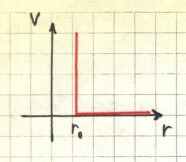
\includegraphics[scale=0.4]{images/1606337089.jpg}

Aquí $r_0$ es $\sigma$ y será la distancia mínima entre dos partículas. Este potencial ilustrado
es sencillamente
\[
	v(r) = \begin{cases}
		\infty \quad r < r_0 \\
		0      \quad r > r_0
	       \end{cases}
\]
Se tienen
\[
	a_2 = \frac{2\pi}{\lambda^3} \frac{r_0^3}{3}
\]
que lleva a $B_2 = 2 \pi r_0^3 / 3$. Se considera a las partículas como esferas duras (bolas de
radio $r_0/2$) entonces $B_2 = 4 v_0$ que conduce a 
\[
	\frac{Pv}{kT} = 1 + 4 v_0 f + ...
\]
y vemos que la $P_{ER} > P_{GI}$.

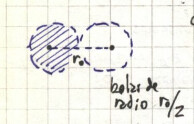
\includegraphics[scale=0.5]{images/1606337092.jpg}

DIBUJO 

\[
	b_2 = \frac{1}{2\lambda^3 V} \int_0^\infty du 4 \pi u^2 f_u = \frac{-1}{2\lambda^3 V} \frac{4\pi\sigma^3}{3}
\]

Sea ahora un potencial de Lenard-jones aproximado.

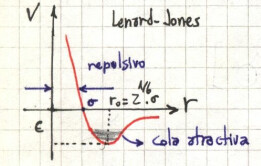
\includegraphics[scale=0.5]{images/1606337096.jpg}

Es algo como
\[
	V(r) =  4 \vare \left[ \Frac{ \sigma }{r}^12 - \Frac{ \sigma }{r}^6 \right]
\]
\[
	V(r) = \begin{cases}
		\infty \quad r < r_0 \\
		\\
		\displaystyle -U_0\Frac{r_0}{r}^b      \quad r > r_0
	       \end{cases}
\]
Entonces el coeficiente es
\[
	a_2 = \frac{2\pi}{\lambda^3} 
	\int_0^{r_0} \: r^2 \: dr + \int_{r_0}^\infty \: ( 1 - \euler^{u_0/(kT)(r_0/r)^b} ) r^2 \: dr 
\]
y aproximaremos van der Waals con $\mu_0/(kT) \ll 1$ (i.e. energía térmica mucho mayor que el pozo de potencial)
de manera que 
\[
	( 1 -  \euler^{u_0/(kT)(r_0/r)^b} ) \approx \frac{\mu_0}{kT} \Frac{r_0}{r}^b
\]
\[
	a_2(T) \approx  \frac{2\pi r_0^3}{\lambda^33} \left( 1 - \frac{u_0}{kT} \right)
\]
\[
	P = \frac{ N k T }{V} \left[ 1 + \frac{2\pi r_0^3}{v} \left( 1 - \frac{u_0}{kT} \right) \right]
	= \frac{ N k T }{V} \left( 1 - \frac{B_2}{v} \right) 
\]
Se puede ir a la ecuación de Van der Waals
\[
	 \left( P + \frac{2\pi r_0^3 u_0}{3v^2} \right) = \frac{kT}{v} \left( 1 + \frac{2\pi r_0^3}{3} \frac{1}{v} \right)
\]
donde en el último término dentro del paréntesis el primer factor es el volumen asociado con el {\it carozo duro}
del potencial y el segundo el volumen específico. Estamos usando la aproximación de gas diluido, es decir
que $ r_0 \ll v^{1/3}$.

Recordando la aproximación usual de $ (1+x)^u \sim 1 + u x $ se logra
\[
	\left( P + \frac{2\pi r_0^3 u_0}{3v^2} \right) \approx 
	\frac{kT}{v} \left( 1 - \frac{2\pi r_0^3}{3} \frac{1}{v} \right)^{-1}
\]
\[
	\left( P + \frac{a}{v^2} \right) (v - b) = k T
\]
de suerte que se tienen
\[
	a =(2/3) \pi r_0^3 u_0
	\qquad 
	b = 2 \pi /3 r_0^3
\]

Podemos relacionar los parámetros $a,b$ de Van der Waals con cosas microscópicas

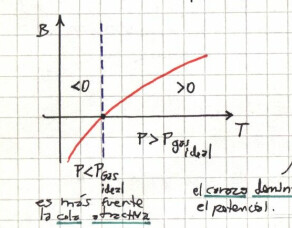
\includegraphics[scale=0.5]{images/1606337115.jpg}

Con este material los problemas 1,3,5,6 pueden encararse.
\notamargen{La flecha cortada en el gráfico este dice que ``partículas coon mucha
energía solo chocan''.}

Lo que sigue a continuación tal vez sea de esferas rígidas o tal vez sea de algo totalmente
diferente. No lo sé.

\[
	Z_3 = \int d^3q_1 \int d^3q_2 \int d^3q_3 \; ( 1 + f_{12} ) ( 1 + f_{13} ) ( 1 + f_{23} )
\]
\begin{multline*}
	Z_3 = 	\int d^3q_1 d^3q_2 d^3q_3 + \int d^3q_1 d^3q_2 d^3q_3 \: f_{12} +
	\int d^3q_1 d^3q_2 d^3q_3 \: f_{13} + \\ \int d^3q_1 d^3q_2 d^3q_3 \: f_{23} +
	\int d^3q_1 d^3q_2 d^3q_3 \: f_{12}f_{13}  + \int d^3q_1 d^3q_2 d^3q_3 \: f_{12}f_{23} + \\
	\int d^3q_1 d^3q_2 d^3q_3 \: f_{13}f_{23} + \int d^3q_1 d^3q_2 d^3q_3 \: f_{12}f_{13}f_{23} 
\end{multline*}
\[
	Z_3 = + + + + + + 
\]
(muchos dibujitos)

Se observa cierta degeneración. Podemos dar los números de ocupación de cada N-grafo
\[
\begin{aligned}
	\{ m_l \} = & (3,0,0) \qquad \text{ 1er N-grafo } \\
	\{ m_l \} = & (1,1,0) \qquad \text{ 2-4 N-grafo } \\
	\{ m_l \} = & (0,0,1) \qquad \text{ 5-8 N-grafo }
\end{aligned}
\]

Son sólo tres conjuntos $\{ m_l \}$ que describen todos los ocho 3-grafos. Sumamos los diferentes permutaciones de 
etiquetas distinguibles de cada conjunto $\{ m_l \}$
\[
	S((3,0,0)) = [  ]^3 = [\lambda^0 V b_1 ]^3
\]
\[
	S((1,1,0)) = []^1[]^1 = 3! [\lambda^0 V b_1 ]^1 [\lambda^3 V b_2 ]^1
\]
\[
	S((0,0,3)) = []^3 = 3! [\lambda^6 V b_3 ]^1
\]
\[
	\sum_{ \{ m_l \} } = 3! \left[ \frac{(V b_1)^3}{3!} + \lambda^3 V^2 b_1 b_2 + \lambda^6 V b_3 \right]
\]

\subsection{hoja suelta --reubicar--}
\[
	\hat{\rho} = \frac{\euler^{\beta \hat{H}}}{Q_N(V,T)} \quad \rightarrow \quad 
	\text{ Tr }(\hat{\rho}) = \frac{1}{Q_N(V,T)} \text{ Tr }(\euler^{\beta \hat{H}})
\]
\[
	1 =  \frac{1}{Q_N(V,T)} \text{ Tr }(\euler^{\beta \hat{H}})
\]
\[
	Q_N(V,T) = \text{ Tr }(\euler^{\beta \hat{H}})
\]

Pero la traza debe evaluarse en alguna base dada,
\[
	\text{ Tr }(\euler^{\beta \hat{H}}) = 
	\int \Bra{\vb{q}_1,..., \vb{q}_N} \euler^{-\beta \hat{H}} \Ket{\vb{q}_1,..., \vb{q}_N} d^{3N}q
\]
\[
	= \int \Bra{\vb{q}_1,..., \vb{q}_N} \euler^{-\beta \hat{H}} 
	\sum_E \Ket{\Psi_E} \braket{\Psi_E | \vb{q}_1,..., \vb{q}_N} d^{3N}q
\]
\[
	= \int  \sum_E \euler^{ -\beta E }  \braket{\vb{q}_1,..., \vb{q}_N | \Psi_E} 
	\braket{\Psi_E | \vb{q}_1,..., \vb{q}_N} d^{3N}q
\]
\[
	\text{ Tr }(\euler^{\beta \hat{H}}) = 
	\int \sum_E \euler^{ -\beta E }  \Psi_E (\vb{q}_1,..., \vb{q}_N ) 
	\Psi_E^*(\vb{q}_1,..., \vb{q}_N ) d^{3N}q
\]
donde $\Ket{\Psi_E}$ son autoestados de energía del $\hat{H}$. Usaremos la función de onda simetrizada y normalizada
\[
	\Psi_E (\vb{q}_1,..., \vb{q}_N )  =
\]
\begin{multline*}
	\Psi_E \Psi_E* = \frac{1}{N!} \sum_{\mathbb{P},\mathbb{P}'} \delta \mathbb{P} u_1(\mathbb{P}_1)
	u_2(\mathbb{P}_2) ... \delta \mathbb{P}' u(\mathbb{P}'_1)(1) u(\mathbb{P}'_2) (2) ... \\
	\sum_{\mathbb{P}} \delta(\mathbb{P}) u_1(\mathbb{P}_1) u_1^*(1) u_2(\mathbb{P}_2) u_2^*(2) ...
\end{multline*}


Una función de onda de $N$ partículas correctamente normalizada y simetrizada
\be
	\Psi (\vb{q}_1,..., \vb{q}_N ) = \frac{1}{\sqrt{N!}} \sum_{ \mathbb{P} } \delta \mathbb{P} \; \mathbb{P}
	\{ u_1(\vb{q}_1) u_2(\vb{q}_2) ... \}
	\label{fun_onda_norm}
\ee
\notamargen{$\mathbb{P}$ es el operador de permutaciones}
donde 
\[
	\Psi_B (\vb{q}_1,..., \vb{q}_N ) = \prod_{i=1}^{n_1} u_1(\vb{q}_1) \prod_{i=n_1+1}^{n_1+n_2} u_2(\vb{q}_2)
\]
es una función para partículas distinguibles (de Boltzmann).

Cada
\notamargen{Estas $\Psi$ son autofunciones del $\hat{H}$.}
\[
	u_{p_i}(\vb{q}_i) = \frac{1}{\sqrt{V}} \euler^{ i \vb{p}_i \cdot \vb{q}_i / \hbar }
\]
es función de onda de la partícula i-ésima en el ninvel energético $e_i$ dado por 
\[
	e_i = \frac{|\vb{p}_i|^2}{2m}
\]

Dado que sumamos en todas las permutaciones de \eqref{fun_onda_norm} es lo mismo permutar coordenadas que vectores
\[
	\Psi (\vb{q}_1,..., \vb{q}_N ) = \frac{1}{\sqrt{N!}} \sum_{ \mathbb{P} } \delta \mathbb{P} \;
	\left( u_{\mathbb{P}_1}(1) u_{\mathbb{P}_2}(2) ... \right) = 
	\frac{1}{\sqrt{N!}} \sum_{ \mathbb{P} } \delta \mathbb{P} \;
	\left( u_1({\mathbb{P}_1}) u_2({\mathbb{P}_2}) ... \right)
\]
\begin{multline*}
	\Psi (\vb{q}_1,..., \vb{q}_N ) \Psi^* (\vb{q}_1',..., \vb{q}_N' ) = \frac{1}{N!} \times \\
	\sum_{\mathbb{P}} \;  \delta \mathbb{P} \; \left(  u_1({\mathbb{P}_1}) u_2({\mathbb{P}_2}) ...\right)
	\sum_{\mathbb{P}'} \;  \delta \mathbb{P}' \; \left(  u_{\mathbb{P}_1}^*(1') u_{\mathbb{P}_2}^*(2') ... \right)\\
	= \frac{1}{N!} \sum_{\mathbb{P},\mathbb{P}'}\delta \mathbb{P} \delta \mathbb{P}'
	\left[ u_1({\mathbb{P}_1}) u_{\mathbb{P}_1}^*(1') u_2({\mathbb{P}_2}) u_{\mathbb{P}_2}^*(2') ... \right]
\end{multline*}

Dado que las permutaciones sólo difieren en el orden de los términos consideramos sólo una permutación repetida $N!$ 
veces, con lo cual 
\[
	\Psi (\vb{q}_1,..., \vb{q}_N ) \Psi^* (\vb{q}_1',..., \vb{q}_N' ) =
	\sum_{\mathbb{P}} \delta \mathbb{P} 
	\left[ u_1({\mathbb{P}_1}) u_{\mathbb{P}_1}^*(1') u_2({\mathbb{P}_2}) u_{\mathbb{P}_2}^*(2') ... \right]
\]
\[
	\Psi (\vb{q}_1,..., \vb{q}_N ) \Psi^* (\vb{q}_1',..., \vb{q}_N' ) =
	\sum_{\mathbb{P}} \delta \mathbb{P}
	\left[ \frac{\euler^{ i \vb{p}_1 \cdot ( \mathbb{P}\vb{q}_1 - \vb{q}_1' )/\hbar} }{V} \times 
	\frac{\euler^{ i \vb{p}_2 \cdot ( \mathbb{P}\vb{q}_2 - \vb{q}_2' )/\hbar}}{V} \times ... \right]
\]
\notamargen{
\[
	\delta \mathbb{P} = \begin{cases}
	                     1 \qquad \text{ bosones } \\
	                     \pm 1 \qquad \text{ fermiones}\\
	                     \text{ (perm par o impar) }
	                    \end{cases}
\]}

Ahora sea el sistema de las $N$ partículas con energía $E$, es decir 
\[
	E = \sum_i^N \; \frac{|\vb{p}_i|^2}{2m} =
	\frac{1}{2m} \left( |\vb{p}_1|^2 + |\vb{p}_2|^2 + ... + |\vb{p}_N|^2 \right)
\]
el estado energético será función de un vector $\vb{P}$
\[
	\vb{P} = (\vb{p}_1, \vb{p}_2, ..., \vb{p}_N )
\]
quiero evaluar 
\[
	\braket{ \{ \vb{q} \} | \euler^{\beta \hat{H}} | \{ \vb{q} \} } =
	\sum_P \euler^{-\beta E(P)} \Psi (\vb{q}_1,..., \vb{q}_N ) \Psi^* (\vb{q}_1',..., \vb{q}_N' )
\]
\notamargen{Suma en todos los $P$ posibles.}
pero esta sumatoria en $P$ es equivalente a 
\[
	\frac{1}{N!} \sum_{\vb{p}_1} \sum_{\vb{p}_2} ... \sum_{\vb{p}_N} 
	\euler^{-\beta/2m \left( |\vb{p}_1|^2 + |\vb{p}_2|^2 + ... + |\vb{p}_N|^2 \right)}
\]

\begin{multline*}
	= \frac{1}{N!} \sum_{\vb{p}_1} \sum_{\vb{p}_2} ... \sum_{\vb{p}_N} 
	\euler^{-\beta/2m \left( |\vb{p}_1|^2 + |\vb{p}_2|^2 + ... + |\vb{p}_N|^2 \right)} \times \\ 
	\sum_{ \mathbb{P} } \delta\mathbb{P} \: \frac{\euler^{ i \vb{p}_1 \cdot ( \mathbb{P}\vb{q}_1 - \vb{q}_1')/ 
	\hbar} }{V} \times \frac{\euler^{ i \vb{p}_2 \cdot ( \mathbb{P}\vb{q}_2 - \vb{q}_2' )/\hbar} }{V}\times ...
\end{multline*}
\[
	= \frac{1}{N!}\sum_{ \mathbb{P} } \delta\mathbb{P} \: \left( 
	\sum_{\vb{p}_1} \frac{\euler^{ -\beta/2m|\vb{p}_1|^2 + i \vb{p}_1 \cdot \vb{r}_1/ \hbar} }{V} \times 
	\sum_{\vb{p}_2} \frac{\euler^{ -\beta/2m|\vb{p}_2|^2 + i \vb{p}_2 \cdot \vb{r}_2/ \hbar} }{V} \times ...
	\right)
\]
donde 
\[
	\vb{r}_i = ( \mathbb{P}\vb{q}_i - \vb{q}_i')
\]

La cuenta entre paréntesis es integrable pasando al continuo con 
\[
	\frac{V}{h^3} \delta \vb{p}_i = 1 \quad \rightarrow \quad \frac{d\vb{p}_i}{h^3} = \frac{1}{V}
\]
\[
	= \frac{1}{N!} \sum_{ \mathbb{P} } \delta\mathbb{P} \: \left( 
	\frac{1}{h^3} \int d\vb{p}_1 \euler^{ -\beta/2m|\vb{p}_1|^2 + i \vb{p}_1 \cdot \vb{r}_1/ \hbar} \times 
	\frac{1}{h^3} \int d\vb{p}_2 \euler^{ -\beta/2m|\vb{p}_2|^2 + i \vb{p}_2 \cdot \vb{r}_2/ \hbar} \times ...
	\right)
\]

Descomponemos cada integral en tres
\[
	I \equiv \left[ \frac{1}{h} \int dp_x \euler^{ -\beta/2m p_x^2 + i p_x r_x/ \hbar} \right] 
	\left[ \frac{1}{h} \int dp_y ... \right] \left[ \frac{1}{h} \int dp_z ... \right]
\]

Usamos que 
\[
	\int dp \euler^{-ap^2} \euler^{-ibp} = \frac{\sqrt{\pi}}{\sqrt{a}} \euler^{-b^2/(4a)}
\]
\[
	I_x = \frac{1}{h} \sqrt{\frac{2\pi m}{\beta}} \euler^{-\frac{2r^2m}{4\beta \hbar^2}} =
	\frac{1}{h} \sqrt{2\pi m kT} \euler^{-\frac{2mkT\pi^2 r^2}{h^2}} = 
	\frac{1}{\lambda} \euler^{-r_x^2\pi /\lambda^2}
\]
\[
	I = I_x I_y I_z = \frac{1}{\lambda^3} \euler^{ -\frac{\pi}{\lambda^2}
	[ (\mathbb{P}q_x-q_x')^2 + (\mathbb{P}q_y-q_y')^2 + (\mathbb{P}q_z-q_z')^2 ]} = 
	\frac{1}{\lambda^3} \euler^{ -\frac{\pi}{\lambda^2} |\vb{r}|^2 }
\]

Luego,
\[
	= \frac{1}{N!} \sum_{ \mathbb{P} } \delta\mathbb{P} \frac{1}{\lambda^{3N}}
	\euler^{ -\frac{\pi}{\lambda^2} |\vb{r}_1|^2 } \times \euler^{ -\frac{\pi}{\lambda^2} |\vb{r}_2|^2 } \times ...
\]

Definimos
\[
	f( \vb{r}_i ) = \euler^{ -\frac{ \pi |\vb{r}_i|^2 }{ \lambda^2 } } \qquad 
	f( \mathbb{P}\vb{q}_i - \vb{q}_i' ) = \euler^{ -\frac{ \pi }{ \lambda^2 }(\mathbb{P}\vb{q}_i - \vb{q}_i')^2 }
\]

Resultando 
\[
	= \frac{1}{N!\lambda^{3N}} \sum_{\mathbb{P}} \delta\mathbb{P} [ f( \mathbb{P}\vb{q}_1 - \vb{q}_1' ) ... 
	f( \mathbb{P}\vb{q}_N - \vb{q}_N' )]
\]
\[
	\braket{ \vb{q}_1,..., \vb{q}_N|\euler^{-\beta\hat{H}}| \vb{q}_1',..., \vb{q}_N' } = 
	\frac{1}{N!\lambda^{3N}} \sum_{\mathbb{P}} \delta\mathbb{P} [ f( \mathbb{P}\vb{q}_1 - \vb{q}_1' ) \times 
	... \times f( \mathbb{P}\vb{q}_N - \vb{q}_N' )]
\]
\begin{multline*}
	\text{ Tr} (\euler^{-\beta\hat{H}}) = \int d^{3N} q
	\braket{ \vb{q}_1,..., \vb{q}_N|\euler^{-\beta\hat{H}}| \vb{q}_1',..., \vb{q}_N' } =\\
	\frac{1}{N!\lambda^{3N}} \int d^{3N}q \sum_{\mathbb{P}} \delta\mathbb{P} [ f( \mathbb{P}\vb{q}_1 - \vb{q}_1' ) 
	\times ... \times f( \mathbb{P}\vb{q}_N - \vb{q}_N' )]
\end{multline*}
\[
	\text{ Tr} (\euler^{-\beta\hat{H}}) = \frac{1}{N!\lambda^{3N}} \int d^{3N}q \sum_{\mathbb{P}} 
	\delta\mathbb{P} \prod_i f( \mathbb{P}\vb{q}_i - \vb{q}_i )
\]

Analizamos la $\sum_{\mathbb{P}}$. Como se suma en todas las permutaciones, tendremos
\[
	\sum_{\mathbb{P}} f(\mathbb{P}{q}_1 - {q}_1) f(\mathbb{P}{q}_2 - {q}_2) ... =
\]
\[
	1 \: f(0) \pm \sum_{i<j} f_{ij} f_{ji} + \sum_{i<j<k} f_{ij} f_{jk} f_{ki} \pm ...
\]
\[
	\text{ 0 permut } \qquad \text{ 1 permut } \qquad \text{ 2 permut }
\]

Veamos la permutación de $q_1$ y $q_2$
\[
	\underbrace{\mathbb{P}}_{=1} (\prod_i f( \mathbb{P}\vb{q}_i - \vb{q}_i ) ) =
	\underbrace{f(\mathbb{P}{q}_1 - {q}_1) f(\mathbb{P}{q}_2 - {q}_2)}_{f_{ij}f_{ji}}
	\underbrace{\prod_{i=3}^N f(q_i - q_i)}_{\prod f(0)=1}
\]
\[
	q_1 \; q_2 \; q_3 \; ... \; q_N
\]
\[
	q_1 \; q_2 \; q_3 \; ... \; q_N
\]

\[
	\underbrace{\mathbb{P}}_{=2} (\prod_i f( \mathbb{P}\vb{q}_i - \vb{q}_i ) ) =
	\underbrace{f( {q}_2 - {q}_1 )}_{f_{ij}} \underbrace{f( {q}_3 - {q}_2 )}_{f_{ki}}
	\underbrace{f( {q}_1 - {q}_3 )}_{f_{jk}}
	\prod_{i=4}^N f(0)
\]
\[
	q_1 \; q_2 \; q_3 \; ... \; q_N
\]
\[
	q_1 \; q_2 \; q_3 \; ... \; q_N
\]

\[
	\underbrace{\mathbb{P}}_{=3} (\prod_i f( \mathbb{P}\vb{q}_i - \vb{q}_i ) ) =
	f( {q}_2 - {q}_1 ) f( {q}_1 - {q}_2 ) f( {q}_4 - {q}_3 ) f( {q}_3 - {q}_4 ) 
	\prod_{i=5}^N f(0)
\]
\[
	q_1 \; q_2 \; q_3 \; q_4 \; ... \; q_N
\]
\[
	q_1 \; q_2 \; q_3 \; q_4 \; ... \; q_N
\]
\[
	\text{ Tr} (\euler^{-\beta\hat{H}}) = \frac{1}{N!\lambda^{3N}} \int d^{3}q 
	\left( 1 \pm \sum_{i<j} f_{ij} f_{ji}  \right)
\]
\notamargen{El $+$ es por bosones y el $-$ por fermiones.}
\[
	f_{ij} = \euler^{ -\frac{\pi}{\lambda^2} |\vb{q}_i - \vb{q}_j|^2} =
	\euler^{ -\frac{\pi}{h} 2\pi k T |\vb{q}_i - \vb{q}_j|^2}
\]

Veamos los límites clásico y el surgimiento de fenómenos cuánticos 
\[
	\text{ CLÁSICO } \qquad v = \frac{V}{N} \ggg 1 \quad \Rightarrow \quad 
	|\vb{q}_i - \vb{q}_j| \gg 1 \qquad T \ggg 1
\]
y por lo tanto
\[
	\euler^{ -\frac{\pi}{h} 2\pi k T |\vb{q}_i - \vb{q}_j|^2} \to 0
\]
\[
	\text{ Tr} (\euler^{-\beta\hat{H}}) = \frac{1}{N!\lambda^{3N}} \int d^{3}q (1) =
	\frac{1}{N!}\Frac{V}{\lambda^3}^N
\]
\[
	\Or(v) \approx 1 \quad \Rightarrow \quad \Or(|\vb{q}_i - \vb{q}_j|) \approx 1 \qquad
	\Or(T) \approx 1
\]
y en este caso es
\[
	\euler^{ -\frac{\pi}{h} 2\pi k T |\vb{q}_i - \vb{q}_j|^2} \to 1
\]
\begin{multline*}
	\text{ Tr} (\euler^{-\beta\hat{H}}) \cong \frac{1}{N!\lambda^{3N}} \int d^{3}q 
	\left( 1 \pm \sum_{i<j} f_{ij} f_{ji}  \right) \\ 
	\cong \frac{1}{N!\lambda^{3N}} \int d^{3}q 
	\left[ \prod_{i<j} (1 \pm f_{ij} f_{ji} ) \right] 
\end{multline*}
\notamargen{Este pasaje vale si $f_{ij} f_{ji}$ es pequeño.}

\begin{multline*}
	\prod_{i<j} ( 1 \pm f_{ij}f_{ji}) = \displaystyle \euler^{\log \prod_{i<j} ( 1 \pm f_{ij}f_{ji}) } =
	\euler^{\displaystyle \sum_{i<j} \log ( 1 \pm f_{ij}f_{ji}) } = \\
	\euler^{\displaystyle -\beta \sum_{i<j}  kT \log ( 1 \pm f_{ij}f_{ji}) } =
	\euler^{\displaystyle -\beta \sum_{i<j}  V_{ij}^{\pm} }
\end{multline*}
donde 
\[
	V_{ij}^{\pm} = -kT\log \left( 1 \pm \euler^{-\frac{\pi}{\lambda^2}|\vb{q}_i - \vb{q}_j|^2} 
	\euler^{-\frac{\pi}{\lambda^2}|\vb{q}_j - \vb{q}_i|^2} \right) =
	-kT\log \left( 1 \pm  \euler^{-2\frac{\pi}{\lambda^2}|\vb{q}_i - \vb{q}_j|^2} \right)
\]

Con $ | \vb{q}_i - \vb{q}_j| \to 0 $ es
\[
	V_{ij}^{\pm} = -kT\log ( 1 \pm 1 ) = \begin{cases}
	                                           -kT\log (2) \quad \text{ bosones } \\
	                                           -kT\log (o^+) \quad \text{ fermiones } 
	                                          \end{cases}
\]

DIBUJO 

El potencial efectivo $\beta V_{ij}$ luce como la Figura


Límite clásico $\to$ no permutación 

Cuando hay overlap de las funciones de onda de las partículas hay que realizar las permutaciones correspondientes.

La simetría (por la indistinguibilidad que hace necesaria la permutación) lleva a términos efectivos de interacción 
repulsivos (FD) o a atractivos (BE).

\subsection{Parte de gases reales (desde carpeta)}

En el límite clásica la $Z$ se factoriza.
Eso explica los apartamientos del comportamiento Boltzmann. El gas ideal cuántico no tiene correlación dinámica,
sino solo las asociadas al carácter de simetría de la función de onda.

\notamargen{En la carpeta estaba la observación de que: ``salteamos la clase de cuánticos 6''}.


\subsection{Otra cosa suelta --reubicar--}

El parámetro de comportamiento siempre es
\[
	\frac{\lambda^3}{v} = \frac{h^3/(2\pi m kT)^{3/2}}{V/N}
\]
donde la longitud de onda térmica $\lambda = h/(2\pi m kT)^{1/2}$ es una medida que da idea de la dispersión de la 
partícula de masa $m$ y temperatura $T$ considerada como onda. El volumen específico $v=V/N$ es el volumen promedio 
ocupado por una partícula. Luego, $\lambda^3$ es una especie de volumen de la partícula considerada como onda.
Si 
\[
	\lambda^3 > v \qquad \text{ Fenómenos de interferencia cuántica }
\]
\[
	\lambda^3 < v \qquad \text{ No hay fenómenos de interferencia cuántica }
\]

GRAFIQUETES

$\lambda$ es una característica del sistema de partículas $(m,T)$
\begin{center}
\begin{tabular}{c c}
$\displaystyle \frac{\lambda^3}{v} \ggg 1 $ & $\displaystyle \frac{\lambda^3}{v} \lll 1 $ \\
Altamente cuántico &  Altamente clásico\\
alta $N/V$ & baja $N/V$\\
baja T & alta T
\end{tabular}
\end{center}

Para Bose el análisis parte de 
\[
	\euler^{-\beta(e-\mu)} < 1 \quad \rightarrow \quad \mu < e \to \mu < 0
\]
\notamargen{gas ideal $e_0=0$, todas con $\vb{p}=0$}
para toda $e$ del sistema, lo cual hará que 
\[
	0 < z < 1 
\]
y
\[
	\frac{N}{V} = \frac{1}{\lambda^3} g_{3/2}(z) + \frac{1}{V} \frac{z}{1-z}
\]

Como $z$ es a lo sumo 1, entonces $g_{3/2}(z)$ está acotada y $g_{3/2}(1)=2.612$
\[
	\frac{\lambda^3}{v} = g_{3/2}(z) + \frac{\lambda^3}{V} \Frac{z}{1-z}
\]

Cuando $z=1$, $g_{3/2}$  ya no puede crecer más; si sube $N$ el remanente $(N-N_e)$ va al estado 
$e_0=0$
\[
	\frac{\lambda^3}{v}(N_e+N_0) = \underbrace{g_{3/2}(z)}_{\lambda^3/V N_e} + \frac{\lambda^3}{V} N_0
\]

Definimos $T_c, v_c$ a partir de $\frac{\lambda^3}{v} = g_{3/2}(1)$ 

Si $ T<T_c$ o $v<v_c$ se tiene 
\[
	\frac{\lambda^3}{v} > g_{3/2}(1) \quad \Rightarrow \quad \frac{\lambda^3}{v} =
	g_{3/2}(1) + \frac{\lambda^3}{V} N_0
\]

Entonces tendremos 
\[
	z = 1 \quad \Rightarrow \quad \mu(T_c) = 0 \quad \Rightarrow \quad T=T_c \quad \Rightarrow \quad  
	\frac{\lambda^3}{v} = 2.612
\]
\[
	T < T_c \quad \Rightarrow \quad \mu(T) = 0 \quad \Rightarrow \quad z = 1 \quad \Rightarrow \quad  
	\frac{\lambda^3}{v} > 2.612
\]
\[
	T > T_c \quad \Rightarrow \quad \mu(T) < 0 \quad \Rightarrow \quad z < 1 \quad \Rightarrow \quad  
	\frac{\lambda^3}{v} < 2.612
\]
\[
	T \gg T_c \quad \Rightarrow \quad \mu(T) \ll 0 \quad \Rightarrow \quad z \ll 1 \quad \Rightarrow \quad  
	\frac{\lambda^3}{v} \ll 1
\]

El $\mu(T)$ luego del condensado $(T<T_c)$ se hace cero con lo cual $z=1$ para todo el intervalo.

Una vez que se tiene el condensado

GRAFICO

\subsection{Cuánticos 6}

comentario estadísticas

modelado de un metal

red de átomos -> gas de fonones -> $c_v$ fonones

Modelos de Debye -> distribución de $\omega$
Einstein -> $\omega = \omega_E$

Modelado de un metal (gas de electrones) -> $c_v$ electrónico

Emisión termoiónica

Tema pequeñas oscilaciones (leer mi resumen)
ver tema de ondas de sonido en sólidos.


%=================================================================================================
\section{Sistemas de partículas indistinguibles y no interactuantes}
% =================================================================================================

\begin{itemize}
 \item no interacción
 \item indistinguibilidad (partículas idénticas)
\end{itemize}

\[
	\hat{H} = \sum_i^N H_i (\vec{q}_i , \vec{p}_i )
\]
\[
	\hat{H} \Psi_E = E \Psi_E \qquad \text{ donde }
\]
\[
	\Psi_E = \prod_{i=1}^{N} u_{e_1}(q_i) \qquad \text{ y } u_{e_1}(q_i)
\]
siendo esta última la solución de una única partícula en el nivel $e_i$ 
y donde $e_i$ es el nivel energético de la partícula 'i'.

El sistema cuántico se describe mediante números de ocupación
\[
	E = \sum_{j=1}^L e_j n_j  \qquad \qquad  N = \sum_{j=1}^L  n_j
\]
siendo $n_j$ el número de partículas en el nivel de energía $e_j$ 
\[
	\Psi_E = \prod_{i=1}^{n_1} u_{e_1}(q_i) \cdot \prod_{i = n_1 + 1 }^{ n_1 + n_2 } u_{e_2}(q_i) \cdot ...
\]

Permutando coordenadas $(\vb{q}_1,\vb{q}_2,...,\vb{q}_N ) \to (P\vb{q}_1,P\vb{q}_2,...,P\vb{q}_N)$ llego a
\[
	\frac{N!}{n_1!n_2!...} = N! \prod_{i=1}^N \frac{1}{n_i!}
\]
diferentes estados. Cada vez que permuto dos partículas en diferentes niveles energéticos cuento un estado extra.

Podemos construir una función de onda cuántica correcta (que no se altere por permutaciones) si respetamos
\[
	| P\Psi |^2 = | \Psi |^2 \quad \text{ dos casos }
\]
\[
	P\Psi = \Psi \qquad \qquad \qquad P\Psi = 
	\begin{cases}
	+ \Psi \text{ número par de permutaciones } \\ 
	- \Psi \text{ número impar de permutaciones } 
	\end{cases}
\]
\[
	\text{ simétrica } \qquad \qquad \qquad \qquad \text{ antisimétrica } 
\]
\[
	\Psi = \sum_P P\Psi \qquad \qquad \qquad \Psi = \sum_P \delta_P P\Psi, \delta_P = \pm 1
\]
\notamargen{Faltaría el coeficiente de normalización}

La antisimetría puede escribirse como determinante de Slater. Además, una función antisimétrica $\Psi$ será nula 
al sumar en 'P' si existe más de una partícula en un mismo nivel energético. Esto equivale a tener dos filas
iguales en el determinante de Slater.
Vemos que el hecho de forzar la simetría de intercambio ha llevado al PRINCIPIO DE EXCLUSIÓN.

\begin{center}
\begin{tabular}{|l|l|l|}
\hline
 & & \\
BOSE-EINSTEIN & $ n_i = 0,1,2, ... , N $ & Cualquier ocupación es válida \\
 (spin entero) & & \\
FERMI-DIRAC  & $ n_i = o, 1 $ & Sólo puede haber a lo sumo una partícula por nivel \\
 (spin semientero) & & \\
\hline
\end{tabular}
\end{center}
\notamargen{La exclusión es $\sum_i^L n_i^2 = N$}

Entonces, dado un conjunto $ \{ n_i \} $ de números de ocupación tendré 

\begin{itemize}
\item 1 estado bosónico : $ \quad \Psi_S = \sum_P P \Psi_{\text{Boltz}}$
\item 1 estado fermiónico : $ \quad \Psi_A = \sum_P \delta_P P \Psi_{\text{Boltz}} 
	\; (\text{ si } N 0 \sum_i^N n_i^2 )$
\item $ \frac{N!}{\prod_i^L n_i!} $ estados de Boltzmann $ \Psi_{\text{Boltz}} = \prod_{i=1}^N u_i(\vec{q}_i) $
\end{itemize}


\subsection{Gas ideal cuántico}

Consideramos $N$ partículas no interactuantes indistinguibles ocupando un volumen $V$ y con energía $E$
Un estado es un conjunto $ \{ n_i^\nu \} $ donde 'i' es nivel energético
\be
	E_\nu = \sum_i e_i n_i^\nu \qquad \qquad N_\nu = \sum_i n_i^\nu
	\label{cond_EN}
\ee

En el microcanónico $ E_\nu = E $ y $ N_\nu = N $ para todo estado $\nu$. Pensamos en cierta estructura 
fina de niveles


donde $g_i$ es el número de subniveles energéticos en la celda 'i' y $n_i$ es el correspondiente número de
partículas en la celda 'i'.

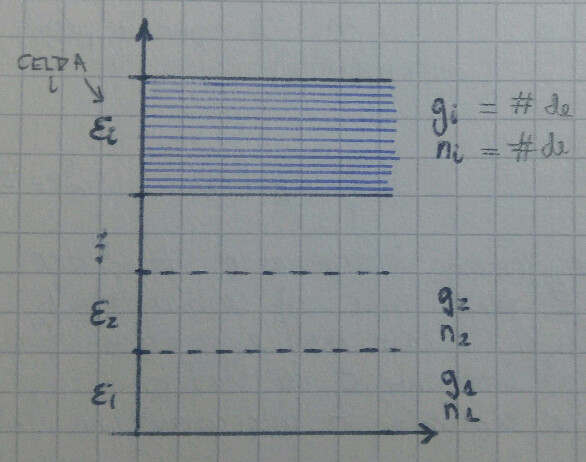
\includegraphics[scale=0.35]{images/1625623752.jpg}

Luego

\[
	\Gamma = \sum_{ \{ n_i \} }' W(\{ n_i \}) = \sum_{ \{ n_i \} }' \prod_i^L  \omega_i 
\]
tendremos
\begin{itemize}
 \item bosones $ \omega_i = \frac{ ( g_i - 1 + n_i)! }{ (g_i - 1)!n_i!} $
 \item fermiones $ \omega_i = \frac{ ( g_i - n_i + n_i )! }{ (g_i - n_i)!n_i!} =
		\frac{ g_i! }{ (g_i -n_i )! n_i!}$
 \item boltzmanniones $ \omega_i = g_i^{n_i} $ y hay que multiplicar por el factor
		$ N! / \prod n_i! $
\end{itemize}
donde $ \omega_i $ es el número de maneras de tener $ n_i $ en $ g_i $ subniveles.
\notamargen{Permutaciones de partículas y paredes (bosones). Permutaciones de partículas y huecos
$g_i \geq n_i $.}

Para el caso de Boltzmann debemos multiplicar por el factor de buen conteo,
\[
	\Gamma = \frac{1}{N!} \sum_{ \{ n_i \} }' \prod_i^L \frac{N!}{\prod (n_i)!}(g_i)^{n_i}
	= \sum_{ \{ n_i \} } \prod_i^L \frac{ (g_i)^{n_i} }{ (n_i)! }
\]

La entropía $S$ es
\[
	S = k \log \sum_{ \{ n_i \} }' W ( \{ n_i \} ) \approx k \log W( \hat{n}_i )
\]
donde se supone que el conjunto $ \{ \bar{n}_i \}$ domina la $ \sum' $. Buscaremos ese conjunto
extremando $S$ sujeto a las condiciones \eqref{cond_EN}.

\[
	\delta ( k\log W( \{ n_i \} ) ) + \alpha \delta N + \beta \delta E = 0
\]
\[
	\bar{n}_i = \frac{ g_i }{ \euler^{ -\beta \mu } \euler^{ \beta e_i } - 1 } \text{ Bose }
\]
\notamargen{Los coeficientes son para las dimensiones. Luego se ve que 
$ \alpha = -\mu / kT \quad \beta = 1 / kT \quad z \equiv \euler^{ \beta \mu} $}
\[
	\bar{n}_i = \frac{ g_i }{ \euler^{ -\beta \mu } \euler^{ \beta e_i } + 1 } \text{ Fermi }
\]
\[
	\bar{n}_i =  g_i \euler^{ \beta \mu } \euler^{ \beta e_i } \text{ Boltzmann }
\]

Esto da el número de partículas por celda energética 'e$_i$' pero interesará por nivel 'g$_i$'.
Entonces dividiremos sobre 'g$_i$' y cambiamos el índice 
\[
	n_j = \frac{1}{z^{-1}\euler^{\beta e_j} + a} \qquad 
	a = \begin{cases}
	 1 \text{ Bose } \\
	 -1 \text{ Fermi } \\
	 0 \text{ Boltmann }
	\end{cases}
\]

La identificación de los coeficientes puede hacerse desde 
\[
	U = TS - pV + \mu N \qquad TS = U  + pV - \mu N
\]
\[
	\frac{S}{k} = \frac{E}{kT} + \frac{pV}{kT} - \frac{\mu}{kT}N \qquad 
	\quad (S=S(E,V,N))
\]
\be
	\frac{S}{k} = \frac{1}{kT} \sum_i n_i e_i + \frac{pV}{kT} - \frac{\mu}{kT} \sum_i n_i
	\label{entropiaSoverk}
\ee

La idea es escribir $ S / k $ en \eqref{entropiaSoverk} de modo que queden explícitas las
$\sum$ que definen $N$ y $E$. Para Bose es 
\[
	\frac{S}{k} = \sum_i n_i \log \left( 1 + \frac{g_i}{n_i} \right) + 
	g_i \log \left( 1 + \frac{n_i}{g_i} \right)
\]
\[
	n_i \log ( n_i + g_i ) - n_i \log ( n_i ) = 
	n_i \log ( n_i \euler^{A} \euler^{Be_i} ) - n_i \log ( n_i )
\]
\[
	\sum_i n_i (A + Be_i) + g_i
\]
\[
	\frac{S}{k} = A \sum_i n_i + B \sum_i e_i n_i + \sum_i g_i \log \left( 1 + \frac{n_i}{g_i} \right)
\]
\[
	A = - \frac{ \mu }{ k T } \qquad \qquad B = \frac{1}{ kT }
\]

\subsection{Microcanónico cuántico (gas ideal) de Boltzmann}

Se puede hacer la cuenta explícitamente.
\[
	\frac{S}{k} = \log \left( \prod_i \frac{}{} \right) =
	\sum_i n_i \log (g_i) - \log n_i!
\]
\[
	\frac{S}{k} \approx 	\sum_i n_i \log \left(\frac{g_i}{n_i}\right) + n_i =
	\sum_i n_i \left( \log (g_i/n_i) + 1 \right)
\]
\[
	N = \sum_i g_i z \euler^{-\beta e_i} = \sum_j z\euler^{-\beta e_j} =
	\frac{1}{h^3} \int d^3p z \euler^{-\beta p^2 / 2m } \int d^3 q =
	\frac{zV}{h^3} (2\pi m k T)^{3/2} = \frac{zV}{\lambda^3}
\]
donde hemos preparado el paso al continuo

En Boltmann es 
\[
	N = \frac{zV}{\lambda^3} \quad \rightarrow \quad z = \frac{\lambda^3}{v} \ll 1 
\]
\[
	E = \frac{3}{2}NkT \qquad \frac{S}{k} = \beta E - N \log( z ) + N
\]


% =================================================================================================
\section{Cuánticos II}
% =================================================================================================

\begin{itemize}
 \item Gas ideal en el gran canónico, entonces el cálculo de $Q_N$ previamente
 \item Gas ideal (Boltmann) en el canónico $\to$ multinomial
\[
	Q_N = \frac{1}{N!} \sum_{n_1}' \sum_{n_2}' ...  \sum_{n_i}' \frac{N!}{n_1!n_2!...}
	\euler^{ -\beta \sum_i n_i e_i }
\]
\[
	Q_N = \frac{1}{N!} \sum_{n_1}' \sum_{n_2}' ...  \sum_{n_i}' \frac{N!}{n_1!n_2!...}
	\prod_i^L \euler^{ -\beta n_i e_i }
\]
\[
	Q_N = \frac{1}{N!} \left( \euler^{-\beta e_1 } + \euler^{ -\beta e_2 } + ... \right)^N
	= \frac{1}{N!} \left( \sum_i \euler^{-\beta e_i } \right)^N =
	\frac{1}{N!} \left( \frac{V}{\lambda^3} \right)^N 
\]
\[
	\log (Q_N) = N \log ( V/\lambda^3 ) - N \log N + 1
\]
\[
	\frac{1}{N} \approx \log \left( \frac{v}{\lambda^3} \right)
\]
\[
	\boxed{ \log Q_N = N \left[ \log \left( \frac{v}{\lambda^3} \right) + 1 \right]}
\]
\item Gas ideal (Fermi y Bose) en el canónico $\to$ {\it hard} $\to$ paso al gran canónico.
\[
	\Xi = \sum_{n=0}^\infty z^N Q_N(V,T)
\]
\[
	\Xi = \sum_{n=0}^\infty \euler^{\beta \mu N} \sum_{n_1}' \sum_{n_2}' ...  \sum_{n_i}' 
	\euler^{ -\beta \sum_i n_i e_i }
\]
y con un {\it magic pass}
\[
	\Xi =  \sum_{n_1}^\infty \sum_{n_2}^\infty ... \sum_{n_i}^\infty
	\euler^{ \beta \mu \sum_i n_i } \euler^{ -\beta \sum_i n_i e_i }
	= \sum_{n_1}^\infty \sum_{n_2}^\infty  ... \sum_{n_i}^\infty \prod_i \euler^{\beta(\mu -e_i )n_i}
\]
\[
	\Xi =  \prod_i^L \left( \sum_{n_i=0}^\infty \euler^{\beta(\mu -e_i )n_i} \right)
\]

Para Boltzmann el gran canónico será 
\[
	\Xi = \sum_{N=0}^\infty \frac{1}{N!} \left( \frac{zV}{\lambda^3}\right)^N
\]
\[
	\Xi(z,V,T) = \begin{cases}
	              \prod_i \frac{1}{1- \euler^{\beta(\mu - e_i)}} \qquad \text{ Bose } \\
	              \prod_i 1 + \euler^{\beta(\mu - e_i)} \qquad \text{ Fermi } \\
	              \euler^{zV/\lambda^3} \qquad \text{ Boltzmann }
	             \end{cases}
\]
\[
	\log \Xi(z,V,T) = \frac{pV}{kT} = \begin{cases}
	              \sum_i -\log (1 - \euler^{\beta(\mu - e_i)} ) \qquad \text{ Bose } \\
	              \sum_i \log (1 + \euler^{\beta(\mu - e_i)} )  \qquad \text{ Fermi } \\
	              \frac{zV}{\lambda^3} = z\sum_i^L \euler^{-\beta e_i} \qquad \text{ Boltzmann }
	             \end{cases}
\]

El número de partículas sale desde 
\[
	\braket{N} = z\dpar{}{z} ( \log \Xi(z,V,T) )
\]
\[
	\braket{N} = \begin{cases}
	             z \sum_i -\frac{1}{1-z\euler^{-\beta e_i}} (-\euler^{-\beta e_i}) =
	             \sum_i \frac{1}{ z^{-1}\euler^{\beta e_i} - 1 } \qquad \text{ Bose } \\
	             z \sum_i \frac{1}{1+z\euler^{-\beta e_i}} (\euler^{-\beta e_i}) =
	             \sum_i \frac{1}{ z^{-1}\euler^{\beta e_i} + 1 } \qquad  \text{ Fermi } \\
	             \frac{zV}{\lambda^3} \qquad \qquad \text{ Boltzmann }
	             \end{cases}
\]
\[
	\braket{n_j} = -\dpar{}{\beta e_j} ( \log \Xi(z,V,T) )
\]
\[ 
	\braket{n_j} = \begin{cases}
	 \displaystyle   -\frac{-1}{1-z\euler^{-\beta e_i}} (-z\euler^{-\beta e_i})(-1) =
			\frac{1}{ z^{-1}\euler^{\beta e_i} - 1 } \qquad \text{ Bose } \\
			\\
	 \displaystyle    \frac{-1}{1+z\euler^{-\beta e_i}} (z\euler^{-\beta e_i})(-1) =
	             \frac{1}{ z^{-1}\euler^{\beta e_i} + 1 } \qquad  \text{ Fermi } \\
	             \\
	 \displaystyle  z \euler^{-\beta e_j} \qquad \qquad \qquad \qquad \qquad \qquad \text{ Boltzmann }
	             \end{cases}
\]
\end{itemize}


\subsection{Funciones termodinámicas}

Todo comienza desde la función de partición

\begin{center}
\begin{tabular}{c|c}
 Fermi &  Bose \\
  & \\
$ \displaystyle \Xi = \prod_i 1 + \euler^{-\beta(e_i - \mu)} $ & 
$ \displaystyle \Xi = \prod_i \frac{1}{1 - \euler^{-\beta(e_i - \mu)}} $ \\
  & \\
$ \displaystyle \beta p V = \sum_i \log (1 + \euler^{-\beta(e_i - \mu)}) $  & 
$ \displaystyle \beta p V = \sum_i -\log (1 - \euler^{-\beta(e_i - \mu)}) $ \\
 & 
\end{tabular}
\end{center}

En gas ideal es, en cartesianas, 
\[
	e = \frac{|\vec{p}|^2}{2m} = ( p_x^2 + p_y^2 + p_z^2 )/2m 
\]
o en esféricas
\[
	e = \frac{p^2}{2m} 
\]

Un gas ideal cuántico generalizará al gas ideal clásico y para valores determinados de los
parámetros ($T,V$ grandes) debería devolver el resultado clásico.
\begin{center}
\begin{tabular}{c|c}
  & \\
$ \displaystyle \braket{N} = \sum_i \frac{1}{\euler^{\beta(e_i - \mu)} + 1} $ & 
$ \displaystyle \braket{N} = \sum_i \frac{1}{\euler^{\beta(e_i - \mu)} - 1} $ \\
  & 
\end{tabular}
\end{center}

El paso al continuo y la integración por partes luego del reemplazo
\[
	\beta e = \frac{\beta p^2}{2m} = \frac{p^2}{2mkT} \cong x
\]
llevará a 
\begin{center}
\begin{tabular}{c|c}
$ \displaystyle \beta p = \frac{1}{\lambda^3} f_{5/2}(z) $ & 
$ \displaystyle \beta p = \frac{1}{\lambda^3} g_{5/2}(z) $ \\
  & \\
$ \displaystyle \frac{\braket{N}}{V} = \frac{1}{\lambda^3} f_{3/2}(z) $ & 
$ \displaystyle \frac{\braket{N}}{V} - \frac{N_0}{V}= \frac{1}{\lambda^3} g_{3/2}(z) $ \\
  & 
\end{tabular}
\end{center}


\notamargen{$ n_0 = \frac{1}{z^{-1} - 1 } = \frac{z}{1-z}$ se va a $\infty$ con 
$z\to 1$ que es $\mu \to 0$.}
Así queda todo en función de 
\[
	f_\nu(z) = \frac{1}{\Gamma(\nu)} \int_0^\infty \frac{x^{\nu-1}}{z^{-1}\euler^x + 1} dx \qquad \text{ y }
	g_\nu(z) = \frac{1}{\Gamma(\nu)} \int_0^\infty \frac{x^{\nu-1}}{z^{-1}\euler^x - 1} dx
\]
\begin{center}
\begin{tabular}{c|c}
  & \\
$ \displaystyle \frac{\lambda^3}{v} = f_{3/2}(z) $ & 
$ \displaystyle \frac{\lambda^3}{v}( N - n_0 ) = g_{3/2}(z) $ \\
  & 
\end{tabular}
\end{center}
\notamargen{$N-n_0$ es la población en los estados excitados.}

Pero tenemos expresiones en términos de $z$
\begin{center}
\begin{tabular}{c|c}
  & \\
$ \displaystyle f_\nu (z) = \sum_{j=1}^\infty \frac{(-1)^{j+1}z^j}{j^\nu} $ & 
$ \displaystyle g_\nu (z) = \sum_{j=1}^\infty \frac{z^j}{j^\nu}  $ \\
  & 
\end{tabular}
\end{center}

Podemos escribir
\begin{center}
\begin{tabular}{c|c}
  & \\
$ \displaystyle \frac{\lambda^3}{v} = z - \frac{z^2}{2^{3/2}} + \frac{z^3}{3^{3/2}}  - ... \qquad $ & 
$ \displaystyle \frac{\lambda^3}{v}( N - n_0 ) = z + \frac{z^2}{2^{3/2}} + \frac{z^3}{3^{3/2}}  - ... \qquad $ \\
  & 
\end{tabular}
\end{center}
con lo cual con $z \ll 1$ nos podemos quedar con los primeros términos.
Asimismo $ n_0 \ll N$.
\begin{center}
\begin{tabular}{c|c}
  & \\
$ \displaystyle \beta p = \frac{z - \frac{z^2}{2^{5/2}} + ... }{v(z - \frac{z^2}{2^{3/2}} + ...)} $ & 
$ \displaystyle \beta p = \frac{z + \frac{z^2}{2^{5/2}} + ... }{v(z + \frac{z^2}{2^{3/2}} + ...)} $ \\
  & \\
$ \displaystyle \frac{pV}{NkT} \cong 1 + \frac{\lambda^3}{v 2^{5/2}} $ & 
$ \displaystyle \frac{pV}{NkT} \cong 1 - \frac{\lambda^3}{v 2^{5/2}} $ \\
  & 
\end{tabular}
\end{center}

Así vemos la corrección positiva (negativa) de origen cuántico.
La presión en el caso de Fermi es mayor (por exclusión) que la ideal; en cambio en
Bose es mayor (condensación).
El gas de Boltzmann tendrá como solución
\[
	\frac{\lambda^3}{v} = z
\]
clásicamente
\[
	\underbrace{ \frac{h^3}{(2 \pi m k T)^{3/2}} }_{ \text{ chico } } 
	\underbrace{\frac{N}{V}}_{ \text{ chico } } = z = \euler^{\mu / kT}
\]
y además como 
\[
	\euler^{\frac{\mu}{kT}} \ll 1 \qquad \frac{\mu}{kT} \ll 0
\]
y entonces
\[
	|\mu| \gg 1, \mu < 0
\]
pero $\mu \equiv \partial U / \partial N$ con lo cual decimos que clásicamente al
aumentar un $\delta N$ tenemos un decrecimiento de la energía $\delta U$ muy grande 
(con $\delta V = \delta S = 0$).
\notamargen{Anoté {\it investigarlo} este asunto.}

Hemos pedido que $\euler^{\beta(\mu - e_i )} < 1 $ para Bose de modo que 
\[
	\beta(\mu - e_i ) < 0 \qquad \mu < e_i \forall i
\]
es el requerimiento para Bose y si $ e_i $ es el ground entonces $ \mu < 0 $.
Si se da que $ \mu \to 0^- $ con $ e_i = 0 $ entonces $ \braket{n_0} \to \infty $.

Para Fermi no hay requerimientos pero 
\[
	0 \leq \braket{n_0} \leq 1
\]

\subsection{Ecuaciones de estado para los gases ideales}

Hay que pasar al continuo
\[
	\frac{pV}{kT} = \log \left[ \Xi (z,V,T) \right] \qquad \qquad 
	\braket{N} = z\dpar{}{z}\left\{ \log \left[ \Xi (z,V,T) \right] \right\}
\]

En el caso de Fermi,
\notamargen{$ x = \beta e = p^2 / 2mkT $}
\[
	\frac{pV}{kT} = \frac{V}{\lambda^3} \frac{4}{3\sqrt{\pi}} \int_0^\infty 
	\frac{x^{3/2}}{z^{-1}\euler^x + 1} = \frac{V}{\lambda^3} f_{5/2}(z)
\]
\[
	\frac{\braket{N}}{V} = \frac{1}{\lambda^3} \frac{1}{2\sqrt{\pi}} \int_0^\infty 
	\frac{x^{1/2}}{z^{-1}\euler^x + 1} = \frac{1}{\lambda^3} f_{3/2}(z)
\]
\[
	f_\nu(z) = \frac{1}{\Gamma(\nu)} \int_0^\infty \frac{x^{\nu - 1}}{z^{-1}\euler^x + 1} =
	\sum_{j=1}^\infty (-1)^{j+1} \frac{z^j}{j^\nu}
\]
y en el caso de Bose
\notamargen{No pasamos al continuo el estado fundamental porque puede diverger}
\[
	\frac{pV}{kT} = \frac{V}{\lambda^3} \frac{4}{3\sqrt{\pi}} \int_0^\infty 
	\frac{x^{3/2}}{z^{-1}\euler^x - 1} - \log ( 1 - z ) = 
	\frac{V}{\lambda^3} g_{5/2}(z) - \log ( 1 - z )
\]
\[
	\frac{\braket{N}}{V} = \frac{1}{\lambda^3} \frac{1}{2\sqrt{\pi}} \int_0^\infty 
	\frac{x^{1/2}}{z^{-1}\euler^x - 1} + \frac{1}{V} \left( \frac{ 1 }{ z^{-1} - 1 } \right) = 
	\frac{1}{\lambda^3} g_{3/2}(z) + \frac{\braket{n_0}}{V}
\]
\[
	g_\nu(z) = \frac{1}{\Gamma(\nu)} \int_0^\infty \frac{x^{\nu - 1}}{z^{-1}\euler^x - 1} =
	\sum_{j=1}^\infty \frac{z^j}{j^\nu}
\]



La energía siempre resulta valer
\[
	\braket{E} = \frac{3}{2}pV
\]
valor que es universal y no depende por lo tanto de la ecuación de estado.

El límite clásico es cuando 
\[
	z^{-1}\euler^{\beta e_i} \ggg 1 \qquad \Rightarrow \qquad \frac{\euler^{\beta e_i}}{z} \ggg 1
\]
y como $ e_i > 0 $ se da $ \euler^{e_i/kT} > 1 $
\[
	z \ll 1 \qquad \euler^{\beta\mu} \ll 1 \qquad \beta\mu \ll 0 \qquad \frac{\mu}{kT} \ll 0
\]
\[
	\mu < 0 \qquad \text{ y } |\mu| \to \infty 
\]
pues $ kT \propto 10^{-19} $ Joules (a 10000 $^\circ$K).
El límite clásico se da con T altas, $ \mu \to -\infty $ y por ello $ z \lll 1$.

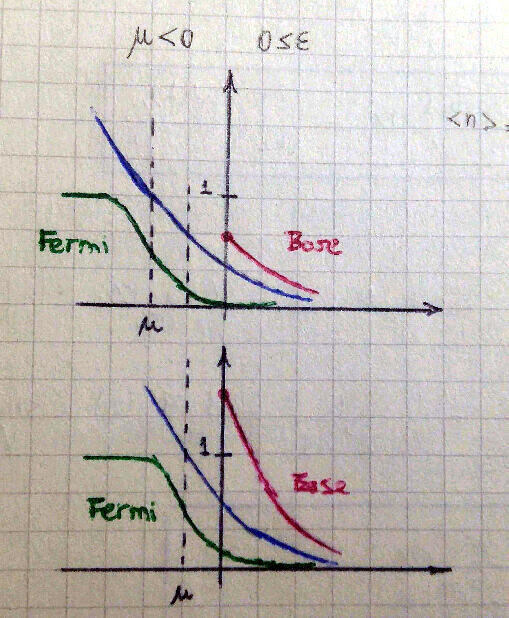
\includegraphics[scale=0.35]{images/1625623872.jpg}

Sea un sistema ideal de bosones $ \mu < 0 $ $ 0 \leq e $
\[
	\braket{n} = \frac{1}{ \euler^{-\beta\mu} \euler^{\beta e} - 1 }
\]
se tiene que para $ e=0 $ y $ \beta\mu = -1 $ es $ \braket{n} = $ 0.582 y para $ e=0 $ y $ \beta\mu = -0.5 $
es $ \braket{n} = $ 1.541

Vemos entonces que el condensado de Bose debe producirse con $ \mu \to 0^{-}$.

\section{Gases cuánticos}

Lo que sigue es un condensado de toda la teoría básica que ya está presente scattereada por aquí y allá.
Obviamente hay que curar y consolidar todo esto.

Se trabajará con gades ideales
\[
	H = \sum_i^N \: H_i
\]
o sea que consideramos no interacción con $N$ partículas indistinguibles. Si la $\Psi^N$ es antisimétrica
estaremos hablando de fermiones (estadística de Fermi-Dirac) y si es simétrica serán bosones, estadística
de Bose-Einstein.

Agregamos una estadística de Maxwell-Boltzmann (teórica). No tendrán una simetría dada; es una aproximación
de alta temperatura de un sistema cuántico.

El conteo de estados, ¿Cómo se realiza?
\begin{enumerate}
 \item Sobre microestados.
 \item Sobre energía $E$, según degeneración $g(E)$.
\end{enumerate}

Tendremos $ E = \sum_i^N \: e_i $ entonces podré factorizar si miro los niveles de energía de una partícula.
Un microestados será definido a través de los números de ocupación,
\[
	n_e = ( n_0, n_1, ..., n_j, ... )
\]
números de ocupación (cantidad de partículas en cada nivel energético). Se tienen 
\[
	\begin{cases}
		\sum_e \: n_e = N = n_0 + n_1 + ... + n_j + ... \\
		\sum_e \: e \: n_e = E
	\end{cases}
\]
y sabemnos que si son bosones se tendrá $n_e=0,1,2,...$ pero para fermiones $n_e=0,1$ (principio de exclusión,
dos partículas no pueden compartir sus números cuánticos). Para Boltzmann consideraremos $ n_e = 0, 1, 2, ...$
distinguibles y metemos el factor $ 1 / N! $. Entonces,
\[
	\begin{cases}
		g(n_e) = 1 \qquad \text{ f, b } \\
		g(n_e) = \frac{ N! }{ \Pi_e \: n_e! } \frac{ 1 }{ N! } \qquad \text{ MB }
	\end{cases} 
\]
pero esto no implica que no haya degeneración en la energía (los casos de fermiones y bosones).
\notamargen{En Bose las combinaciones que me puedo armar son las que harán la función de onda simétrica.}

Las funciones de partición 
\[
	Q_N(V,T) = \sum_{ \{n_e\} } \: \euler^{ -\beta E(n_e) } g(n_e),
\]
pero sujeta a que $ \sum n_e = N $. Para Maxwell-Boltzmann la $ g(n_e) $ quedará un binomio de Newton,
entonces $ Q_N = Q^N / N! $.

Para FD/BE la condición $ \sum n_e = N $ hace complicar la cuenta; nos vamos al gran canónico donde
es mucho más sencilla la cosa porque desaparece esa constraint y entonces
\[
	Q(z,V,T) = \sum_{N=0}^\infty \: z^N Q_N(V,T) =
	\sum_{N=0}^\infty \: z^N \sum_{ \{n_e\} } \: \euler^{ -\beta \sum_e \: e \: n_e }
\]
Se descorrelacionan los números de ocupación y 
\[
	\sum z^{n_0 + n_1 + ...} \sum \euler^{ -\beta ( \: e_0 \: n_0 + e_1 \: n_1 + ... ) } =
	\sum_{n_0} \: z {\euler^{-\beta e_0}}^{n_0} \: \sum_{n_1} \: z {\euler^{-\beta e_1}}^{n_1} ...
\]
y resulta
\[
	\prod ( \sum_{n} \: z {\euler^{-\beta e}}^{n} )
\]
donde $ n=0,1$ para fermiones y $n=0,1,2,...$ para bosones.
Entonces tendremos, respectivamente
\[
	Q(z,V,T) = \begin{cases}
		\displaystyle \prod_e \: \frac{1}{1-z\euler^{\beta e}} \\
		\\
		\displaystyle \prod_e \:  1 + z\euler^{-\beta e}
	\end{cases}
\]
donde en la primer expresión (bosones) se ha usado que $ | z \euler^{-\beta e} | < 1 $ para toda $e$.
\notamargen{Para gases ideales sin spin es $|z|<1$.}

\[
	\beta P V = \begin{cases}
		\displaystyle - \sum_e \: \log ( 1-z\euler^{\beta e} ) \\
		\\
		\displaystyle \sum_e \: \log( 1 + z\euler^{-\beta e} )
	\end{cases}
\]

\[
	N = \begin{cases}
		\displaystyle \sum_e \: \frac{1}{z^{-1}\euler^{\beta e} - 1 } \\
		\\
		\displaystyle \sum_e \: \frac{1}{z^{-1}\euler^{\beta e} + 1 }
	\end{cases}
\]

Recordemos que estamos sumando siempre sobre los niveles energéticos de una sola partícula (sus estados
cuánticos). El número medio de ocupación de cada nivel será
\[
	\vm{n_e} = \frac{1}{Q} \sum_{N=0}^\infty \: z^N \sum_{ \{ n_e\} } n_e \: \euler^{ -\beta \sum_e n_e e }
	= - \frac{1}{\beta} \dpare{ \log Q(z,V,T) }{e}{N,V,\text{ todos los otros $e$}} 
\]
\[
	\vm{n_e} = \frac{ 1 }{ z^{-1} \euler^{ \beta e } \mp 1 }
\]
siendo el primer signo para bosones y el segundo para fermiones.

\subsection{cuentas del paso discreto-continuo}

Consideramos la aproximación de que
\[
	p = \frac{2\pi\hbar}{\ell}( n_x, n_y, n_z ) \qquad \qquad 
	d^3p = \Frac{2\pi\hbar}{\ell}^3
\]
y esto último es el volumen por punto. Luego, el número de puntos por unidad de volumen es $ L^3/h^3 $.
Entonces,
\[
	\sum_p u  \longrightarrow \frac{L^3}{h^3} \int d^3p \longrightarrow  \frac{4 \pi L^3}{h^3} \int p^2 dp
\]
\notamargen{Si depende del módulo puede pasarse fácilmente a esféricas.}

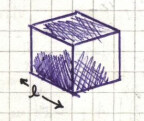
\includegraphics[scale=0.5]{images/1606329596.jpg}

Pero también puedo querer integrar en energía, entonces usamos $ m de = p dp $ que viene de $ e = p^2 / (2m)$
(relación de dispersión no relativista).
\[
	\frac{4 \pi L}{h^3} \int m \sqrt{ 2 m E } (\ldots) de = \int g(e) \: de (\ldots)
\]
donde la densidad de estados es
\[
	g(e) = \frac{4 \pi L}{h^3} m \sqrt{2 m E }.
\]

En $D=2$ dimensiones el factor que se hace cargo de los puntos en una superficie será $A^2$,
\[
	\frac{A^2}{h^2} \int d^2p (\ldots) \qquad  
	\frac{2 \pi A^2}{h^2} \int p dp (\ldots) = \frac{2 \pi A^2}{h^2} \int m de (\ldots)
\]
y entonces,
\[
	g(e) = \frac{2 \pi L^2}{h^2}m.
\]

En $D$ dimensiones tendremos $ g(e) \propto L^D e^{D/2-}$.

Recordemos que aquí siempre estamos en que $g(e)$ es el número de autoestados con energía comprendida
entre $e$ y $e+de$.







% \bibliographystyle{CBFT-apa-good}	% (uses file "apa-good.bst")
% \bibliography{CBFT.Referencias} % La base de datos bibliográfica

\end{document} 
